\section{Conclusiones}


El proyecto ha proporcionado una plataforma invaluable para desarrollar
habilidades esenciales en el diseño e implementación de redes de área local,
enfocándose particularmente en los aspectos de conmutación y enrutamiento. El
éxito del proyecto es una clara demostración de la capacidad de diseñar e
implementar una infraestructura de red compleja, que es una habilidad esencial
en la era digital actual.
\\

Por un lado, hemos diseñado y desplegado una arquitectura de red de tres capas
en Bogotá y una arquitectura Core/Collapsed en Medellín, proporcionando
valiosos aprendizajes sobre la implementación de diversas arquitecturas de red
y su impacto en la capacidad de manejo de tráfico de la red y la conectividad
entre localidades. El diseño e implementación de estas arquitecturas de red han
brindado una comprensión más profunda de los conceptos de conmutación,
esenciales para el funcionamiento efectivo de cualquier red.


\begin{figure}[H]
    \centering
    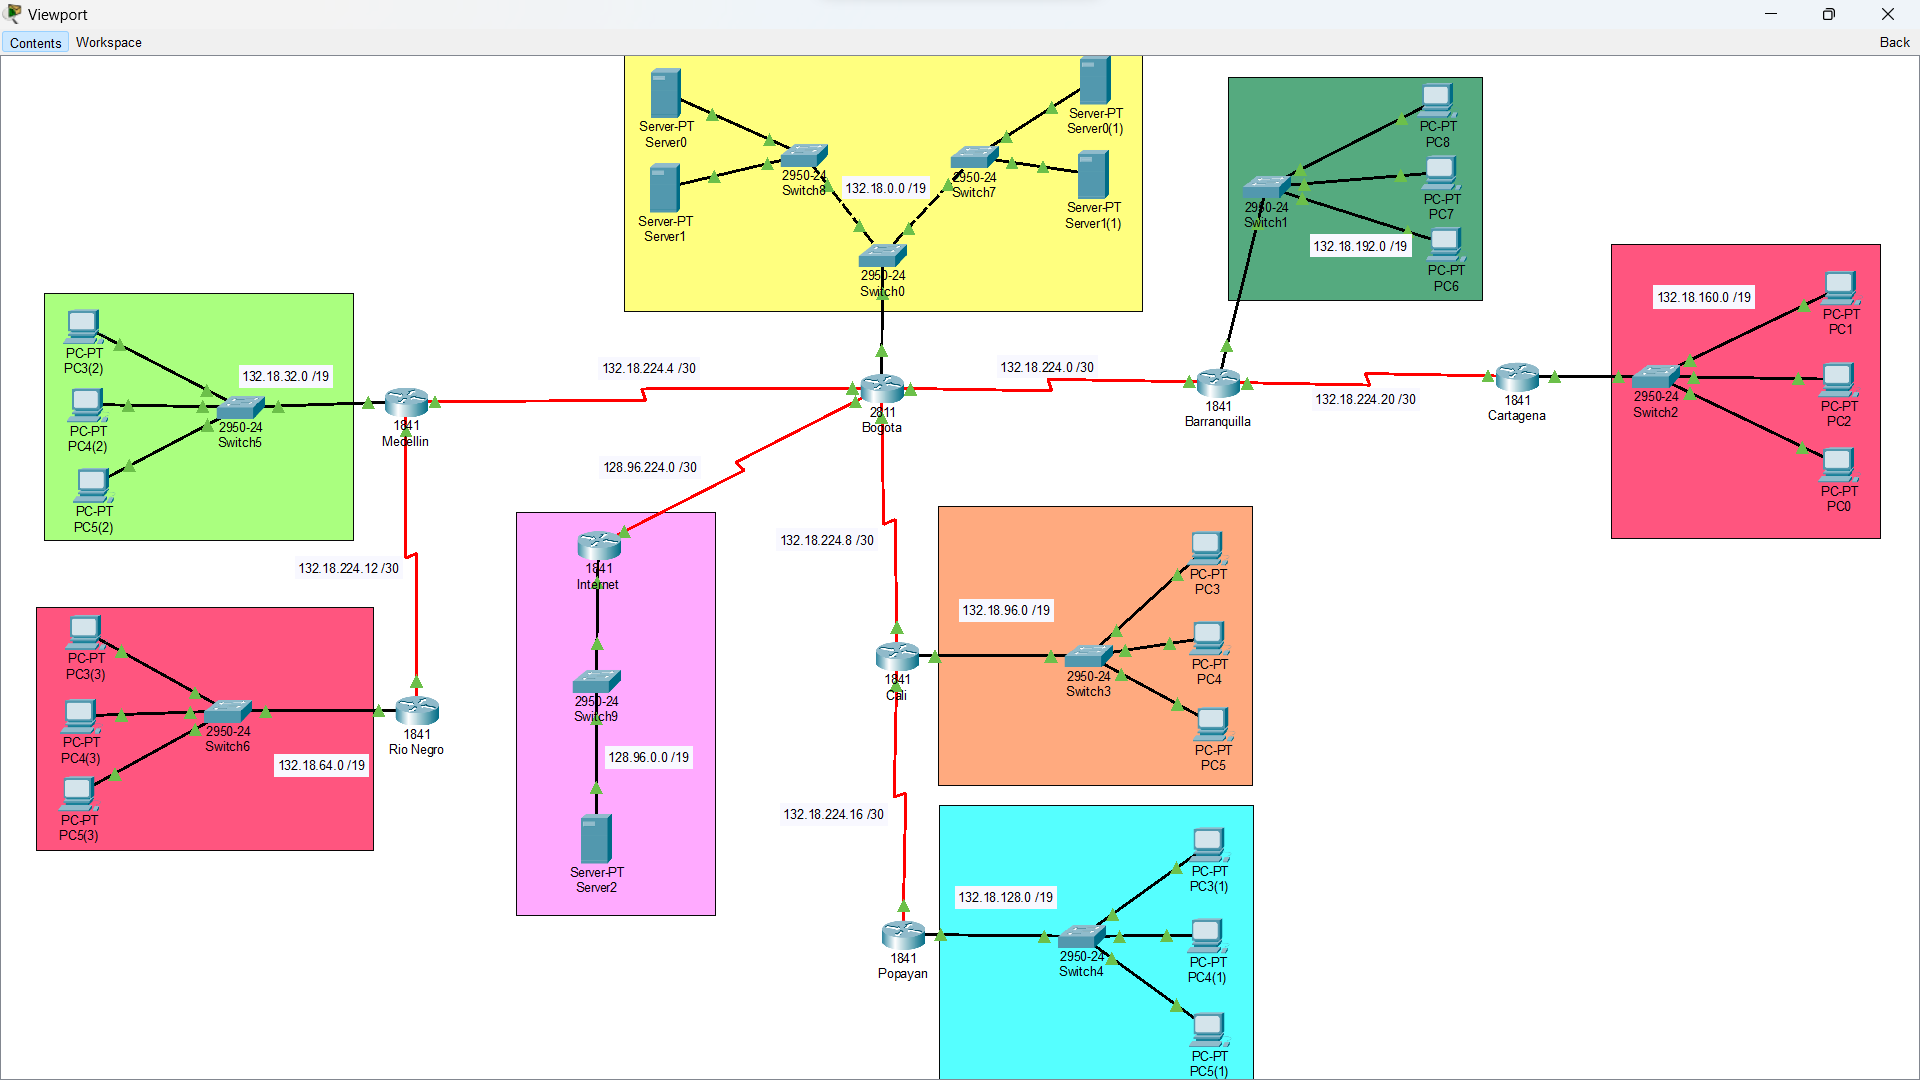
\includegraphics[width=0.7\textwidth]{Figures/4. Conclusions/final_result.png}
    \caption{Topología Completa de la red}
    \label{fig: Topologia Completa de la red}
\end{figure}


Por otro lado, al implementar el esquema de direccionamiento VLSM y el
protocolo de enrutamiento OSPF, hemos obtenido una experiencia práctica en el
manejo de técnicas de enrutamiento, que son cruciales para dirigir el tráfico
de red de manera eficiente. Esta experiencia práctica en enrutamiento ha
proporcionado una comprensión más profunda de cómo se maneja el tráfico de red,
permitiendo una mayor optimización y eficiencia en el diseño de redes.
\\

Además, otro aspecto fundamental de este proyecto fue la implementación de
Network Address Translation (NAT). NAT es crucial para conservar el espacio de
direcciones IP y también para proporcionar seguridad adicional a la red interna.
En nuestro caso, lo utilizamos para permitir que los diversos nodos de la red se
comuniquen con Internet, utilizando una dirección IP pública. Esto no sólo
preservó nuestras direcciones IP internas, sino que también permitió a los
nodos de la red acceder a recursos en Internet de manera eficiente. La
implementación exitosa de NAT proporcionó una experiencia práctica valiosa en
esta técnica esencial de enrutamiento y destacó su importancia en el diseño e
implementación de redes de área local.
\\

En términos de aprendizaje y desarrollo de habilidades, este proyecto ha sido
inmensamente provechoso. Ha permitido aplicar conocimientos teóricos en un
escenario práctico y realista, y ha demostrado que la teoría puede traducirse
en prácticas de red eficaces y eficientes. Como resultado, estamos en una mejor
posición para abordar futuros desafíos de diseño e implementación de redes.
\\

En resumen, al final de este proyecto, no solo hemos entregado una red funcional
y robusta, sino que también hemos adquirido y perfeccionado habilidades
esenciales en el diseño e implementación de redes de área local, con un enfoque
particular en la conmutación y el enrutamiento. Estas habilidades y
conocimientos serán valiosos para afrontar futuros desafíos en el campo de las
redes.